\section{Maximal Monotone Operators in Real Hilbert Spaces}

\subsection{Multivalued Operators}

In this section we will introduce a class of multivalued operators
in $\RR$-Hilbert spaces called maximal monotone operators and study
some of their properties. The theory of gradient flows is based on the class 
of these operators. We proof a criterion for these operators to be 
maximally monotone and use this condition to present a few examples.

\begin{definition}
	A multivalued operator $ A $ in $ \rH $ is a mapping $ A:\rH \ra \rP(\rH)$,
	where $ \rP $ denotes the powerset. 
	The domain of $ A $ is defined by the set $ D(A):=\{x\in \rH \sep A(x) \neq \emptyset\} $ and the range of $ A $ is defined by 
	$ R(A):=\{y\in\rH \sep \exists x \in \rH \st y \in A(x) \} $.
	The mapping $ A $ is single valued, if all elements in the domain of $ A $
	are mapped to singletons.
\end{definition}

Throughout this paper we will make the following simplifications:
For any $ x \in \rH $ we write $ Ax $ as short hand for $ A(x) $, and 
we identify single valued operators with self-mappings in $ \rH $,
i.e. functions of the form $ \rH\ra\rH $. 
We assume $ A\eta $ is any value $ \xi\in A\eta $ for $ \eta\in D(A) $ 
unless specified otherwise. \medskip

It is useful to relate multivalued operator with their graphs in $ \rH\times \rH $. 
This is because set inclusion will endow the set of multivalued operators in 
$ \rH $ with a partial order.

\begin{definition}
	Let $ A $ be a multivalued operator in $ \rH $.
	The graph of $ A $ is defined by the set 
	$ \{(\eta,\xi) \sep \eta\in D(A),\; \xi\in A\eta\} $.
	We identify the multivalued operator $ A $ with its own graph. 
\end{definition}

We need multivalued operators to be compatible with the vector space structure of 
$ \rH $. This motivates the following definition.

\begin{definition}
	Let $ A $ and $ B $ be multivalued operators in $ \rH $ and $ \lambda \in \RR$ any real value. We construct the following multivalued operators in $ \rH $:
	\begin{itemize}
		\item The sum $ A+B $ is defined by $ (A+B)x:=\{y+z \sep y \in Ax,\; z \in Bx\} $ for all $ x\in\rH $, with the domain given by the intersection $ D(A)\cap D(B) $.
		\item The scalar multiple $ \lambda A $ is defined by 
		$ \lambda Ax:=\{\lambda y \sep y \in Ax\} $ for all $ x\in\rH $, 
		whose domain coincides with that of $ A $.
		\item The inverse $ A^{-1} $ of $ A $ is defined by its graph 
		$ A^{-1}:=\{(y,x) \sep (x,y) \in A\} $. The domain and range of $ A^{-1} $ 
		coincide with the ones from $ A $ but interchanged, 
		this means we have that $ D(A^{-1}) = R(A) $ and $ R(A^{-1}) = D(A) $.
	\end{itemize}
\end{definition}

In the Hilbert space $ \RR $ a mapping $ f:\RR\ra\RR $ is monotonically 
increasing if and only if 
it satisfies for the following inequality
\begin{align*}
	\big(f(x)-f(y)\big)\cdot \big(x-y\big)\geq 0
	\qquad \forall x,y\in\RR.
\end{align*} 
This notion of monotonicity can be generalised to any $ \RR $-Hilbert space.

\begin{definition}
	We say a multivalued operator $ A $ in $ \rH $ is monotone, 
	if it fulfils the following inequality
	\begin{align*}
		\inner{\xi_1-\xi_2}{\eta_1-\eta_2}\geq 0
		\qquad \forall (\eta_1,\xi_1),(\eta_2,\xi_2)\in A.
	\end{align*}
\end{definition}

\begin{lemma}\label{lemma:char of mon op}
	Let $ A $ be a multivalued operator in $ \rH $.
	Then $ A $ is monotone if and only if
	for all $ \lambda>0 $ the following inequality holds true
	\begin{align}\label{equation:char of mon op}
		\norm{\eta_1-\eta_1}\leq 
		\norm{(\id+\lambda A)\eta_1-(\id+\lambda A)\eta_2}
		\qquad\forall \eta_1,\eta_2\in D(A).
	\end{align}
\end{lemma}
\begin{proof}
	First suppose the inequality \eqref{equation:char of mon op} 
	holds true. Thus by squaring and restructuring the equations
	we get the equivalent statement
	\begin{align*}
		-\lambda^2 \norm{A\eta_1-A\eta_2}^2\leq 2\lambda 
		\inner{A\eta_1-A\eta_2}{\eta_1-\eta_2},
	\end{align*}
	If we divide by $ \lambda $ and take the limit $ \lambda\se 0 $,
	we get that $ A $ is monotone. On the other hand, if $ A $ is
	monotone, we can reverse the arguments to see that the inequality
	\eqref{equation:char of mon op} is correct.
\end{proof}

\begin{remark}
	Lemma \ref{lemma:char of mon op} shows how the notion of a monotone
	multivalued operator can be extended to include Banach spaces. This
	generalization is investigated in papers such as \cite{10.2307/2373376}. 
\end{remark}

Of particular interest are the maximal elements in the set of monotone 
multivalued operators in $ \rH $ that are partially ordered by the set inclusions
of their graphs.

\begin{definition}
	A monotone multivalued operator $ A $ in $ \rH $ is maximally monotone, if its graph is 
	inclusion-wise maximal in the set of graphs of monotone multivalued operators in $ \rH $. 
	This means that if $ B $ is a monotone multivalued operator in $ \rH $
	with $ A\subseteq B $, then $ A=B $. 
\end{definition}

\begin{remark}\label{remark:char graph el}
	The graph of a maximally monotone operator $ A $ has an equivalent
	definition, on which this semester project will rely on many times. Namely for 
	$ (x,y)\in\rH \times \rH $ we have
	\begin{align}\label{eq1:remark:char graph el}
		(x,y)\in A
		\qequiv
		\inner{y-\xi}{x-\eta}\geq 0
		\qquad\forall (\eta,\xi)\in A.
	\end{align} 
\end{remark}

With the condition \eqref{eq1:remark:char graph el} 
we can build other maximally monotone
operators from an existing one.

\begin{example}\label{example:easy examples of max mon op}
	If $ A $ is a maximally monotone operator on $ \rH $, then so to is
	the scalar multiple $ \lambda A $ for all $ \lambda>0 $ and the inverse
	$ A^{-1} $. \smallskip
	
	In general the same cannot be said about the finite sum of maximally 
	monotone multivalued operators in $ \rH $, as the intersection
	of their domains may be empty. Although there are conditions on the domain
	that permit the aforementioned sum to be maximally monotone 
	(cf. \cite[Chapter 2.6]{brezis1973ope}).
\end{example}

A maximally monotone multivalued operator imposes structural constraints 
on the image of individual elements.

\begin{lemma}\label{lemma:mapped element is weak cl and conv}
	Let $ A $ be a maximally monotone operator in $ \rH $  and
	$ \eta\in D(A) $. Then the set $ A\eta $ is convex and weakly closed 
	for all $ \eta \in D(A) $. In addition for any
	$ \eta_1,\eta_2\in D(A) $ we have
	that $ \Int A\eta_1\cap \Int A\eta_2=\emptyset $, whenever $ \eta_1\neq \eta_2 $.
\end{lemma}
\begin{proof}
	"$ A\eta $ is convex": For all  $ \theta\in[0,1] $ and $ \xi_1,\xi_2\in A\eta $
	we have $ \theta\xi_1+(1-\theta)\xi_2\in A\eta $, since the value satisfies
	the condition \eqref{eq1:remark:char graph el} by the following computation
	\begin{align*}
		\begin{split}
			\inner{\theta \xi_1 + (1-\theta) \xi_2 -y}{\eta-x}
			&=\inner{\theta (\xi_1-y) + (1-\theta) (\xi_2 -y) }{\eta-x}\\
			&=\theta\inner{\xi_1-y}{\eta-x}
			+(1-\theta)\inner{\xi_2 -y}{\eta-x}\\
			& \geq 0
		\end{split}
		\qquad
		\forall (x,y)\in A.
	\end{align*}
	"$ A\eta $ is weakly closed": Let $ (\xi_n)_{n\in\NN}\subseteq A\eta$ 
	be any sequence such that $ \xi_n\ha \xi $ for some $ \xi\in\rH $. 
	Then $ \xi\in A\eta $, as the value satisfies the condition
	\eqref{eq1:remark:char graph el} by the following calculation
	\begin{align*}
		\inner{\xi-y}{\eta-x}
		=\lim_{n\ra\infty}\inner{\xi_n-y}{\eta-x}
		\geq 0
		\qquad
		\forall (x,y)\in A.
	\end{align*}
	"$\Int A\eta_1\cap \Int A\eta_2=\emptyset$": Suppose there exists
	$ \xi\in\rH $ and $ \varepsilon>0 $, such that every $ x\in\rH $ with
	$ \norm{x}<\varepsilon $ satisfies $ \xi+x\in A \eta_1\cap A\eta_2 $.
	Then as $ A $ is maximally monotone we see
	\begin{align*}
		\inner{x}{\eta_1-\eta_2}
		=\inner{(\xi+x)-\xi}{\eta_1-\eta_2}
		\geq 0.
	\end{align*}
	As this inequality must hold for all elements $ x $ in a neighbourhood
	of $ 0 $, we deduce that the identity $ \eta_1=\eta_2 $ must stand.
\end{proof}

We will see in Theorem \ref{theorem:res is proj in limit and dom is conv},
in combination with example \ref{example:easy examples of max mon op},
that a maximally monotone operator even imposes structural constraints 
on its domain and range.\smallskip

Next we present a criterion for a multivalued operator to be
maximally monotone. This proposition will require the use of the
following theorem, a proof of which can be found in 
\cite[Theorem 2.1]{brezis1973ope}.

\begin{theorem}\label{theorem:monotone extension}
	Let $ C $ be a closed convex set in $ \rH $ and $ A $ a monotone operator in $ \rH $.
	For all $ y \in \rH $ there exists $ x\in C $ such that
	\begin{align*}
		\inner{\xi + x}{\eta - x}\geq \inner{y}{\eta - x}
		\quad \forall (\eta,\xi) \in A.
	\end{align*}
\end{theorem}

This theorem lets us state a useful 
criteria for a multivalued operator to be maximally monotone.
In fact we will need these conditions for the examples at the end of this section.

\begin{proposition}\label{proposition:criteria for max mon}
	Let $ A $ be a multivalued operator in $ \rH $. Then the following
	are equivalent
	\begin{enumerate}[label=(\roman*)]
		\item $ A $ is maximally monotone.
		\item $ A $ is monotone and $ R(\id + A)=\rH $.
	\end{enumerate}
\end{proposition}
\begin{proof}
	"(i) $\Ra$ (ii)":  
	If we set $ C=\rH $ in theorem \ref{theorem:monotone extension}, 
	then for all $ y\in\rH $ there exists $ x\in\rH $ with
	\begin{align*}
		\inner{\xi + x}{\eta - x}\geq \inner{y}{\eta - x}
		\quad \forall (\eta,\xi) \in A.
	\end{align*}
	By condition \eqref{eq1:remark:char graph el} we have
	that $ y-x\in Ax $ and thus
	$ y\in R(\id+ A) $. This proves $ R(\id+A)=\rH $.\smallskip
	
	"(ii) $\Ra$ (i)": Let $ B $ be a monotone multivalued operator 
	on $ \rH $ such that $ A\subseteq B $. By assumption for all 
	$ (\eta,\xi)\in B $ 
	there must exist $ z\in D(A) $ satisfying 
	$ \eta+\xi\in z+Az \subseteq z+Bz $. Clearly we have 
	$ \eta+\xi\in \eta+B\eta $.
	Then by using the monotonicity of $ B $, we compute
	\begin{align*}
		0\leq \inner{(\eta+\xi-z)-(\eta+\xi-\eta)}{z-\eta}=-\norm{\eta-z}^2\leq 0.
	\end{align*}
	This shows $ \eta = z $ and thus $ (\eta,\xi)\in A $. Then 
	$ A $ is maximally monotone as $ A=B $.\smallskip
\end{proof}

Of independent interest is that any multivalued monotone 
operator in $ \rH $ can be extended
to a maximally monotone operator. The extension of the domain 
can be restricted to at most the closure of the convex hull 
of the monotone operator.

\begin{corollary}\label{corollary:max mon ext}
	Let $ A $ be a monotone multivalued operator in $ \rH $. 
	There exists some maximally
	monotone operator $ B $ in $ \rH $ with $ A\subseteq B $ 
	and $ D(B)\subseteq \overline{\conv D(A)}$.
\end{corollary}
\begin{proof}
	Let us define the set $ \rD $ of all monotone multivalued
	operators $ B $ in $ \rH $ with $ A\subseteq B $ 
	and $ D(B)\subseteq \overline{\conv D(A)}$. The
	set is endowed with the partial order of the graphs of 
	multivalued operators in $ \rH $. The set $ \rD $
	is non-empty as it contains $ A $. Thus by
	Zorn's Lemma, there exists a maximal element $ B$ in $\rD $.\smallskip
	
	We claim that $ B $ is maximally monotone. Indeed 
	if we set $ C=\overline{\conv D(A)} $ in theorem 
	\ref{theorem:monotone extension}, 
	then for all $ y\in\rH $ there exists $ x\in C $ with
	\begin{align*}
		\inner{\xi + x}{\eta - x}\geq \inner{y}{\eta - x}
		\quad \forall (\eta,\xi) \in B.
	\end{align*}
	As $ B $ is maximal in $ \rD $, we have
	that $ y-x\in Bx $ and thus
	$ y\in R(\id+ B) $. From this we deduce $ R(\id+B)=\rH $.
	So by proposition \ref{proposition:criteria for max mon}
	we have that $ B $ is maximally monotone.
\end{proof}

\begin{remark}
	One may wonder if in corollary \ref{corollary:max mon ext},
	the domain of $ B $ can be restricted to a smaller
	set than $ \overline{\conv D(A)} $. We will see in
	theorem \ref{theorem:res is proj in limit and dom is conv}
	that this is not true.
\end{remark}

With proposition \ref{proposition:criteria for max mon} it is possible
to count some examples of maximally monotone operators.

\begin{example}\label{exampel:mon R funct op}
	Let $ f:\RR \ra \RR$ be a non-decreasing mapping. Define 
	the multivalued operator $ A $ in $ \RR $ by 
	$ A\eta:=[f(\eta-),f(\eta+)] $ for all $ \eta\in \RR $,
	with $ f(\eta\pm):=\lim_{h\se 0}f(\eta\pm h) $. Clearly
	$ R(A) $ is a closed interval in $ \RR $ and thus 
	$ \idm_{\RR}+A $ is a surjective multivalued operator
	and it is monotone as $ f $ is non-decreasing.
	Thus by proposition \ref{proposition:criteria for max mon}
	we know that $ A $ is maximally monotone.
\end{example}

\begin{example}\label{example:map max mon op from H to L2}
	There is a mapping 
	$ \ltwomap $ from maximally monotone
	operators in $ \rH $ into maximally monotone operators in the 
	$ \RR $-Hilbert space\footnote{See definition 
	\ref{definition:lp space in hilbert space}} $ \ltwo $.
	For any maximally monotone operator $ A $ in $ \rH $ we define
	the multivalued operator $ \ltwomap A $ by
	\begin{align*}
		\ltwomap Af=\{u\in\ltwo \sep u(t)\in Af(t)\text{ for a.e. }t\in [0,T]\}
		\qquad\forall f\in D(\ltwomap A),
	\end{align*}
	where the domain of $ \,\ltwomap A $ is defined by 
	$ \{f\in\ltwo\sep f(t)\in D(A)\text{ for a.e. }t\in [0,T] \}$. 
	To show that $ \ltwomap A $ is maximally monotone,
	by proposition \ref{proposition:criteria for max mon}
	it suffices to verify that $ \ltwomap A $
	is monotone and $ R(\idltwo+\ltwomap A)=\ltwo $.
	Then $ \ltwomap A $ is indeed monotone, since for all 
	$ (f_1, u_1),(f_2,u_2)\in\ltwomap A $ we see
	by the monotonicity of $ A $ that
	\begin{align*}
		\ltwoinner{u_1-u_2}{f_1-f_2}
		=\int_0^T
		\inner{u_1-u_2}{f_1-f_2}\,dt
		\geq 0.
	\end{align*}
	Moreover it holds that $ R(\idltwo+\ltwomap A)=\ltwo $,
	since for any
	$ u\in\ltwo $ there exists for almost all $ t\in[0,T] $
	some $ f(t)\in D(A) $ with $ u(t)=f(t)+Af(t) $.
	We have that $ f\in \ltwo $ since
	by lemma \ref{lemma:res is contr onto dom} we know that
	$ \norm{f(t)}\leq \norm{u(t)} $ for almost all $ t\in[0,T] $
	and thus by the dominated convergence theorem we infer the claim. 
	Furthermore $ f\in D(\ltwomap A) $ and
	$ u=f+\ltwomap A f $.
\end{example}

%% Interesting conseuqeunce
%\begin{remark}
%	If we apply the operator $ \ltwomap $ consecutively 
%	$ k $ times for $ k\geq 1 $, then \textbf{replace
%	$ \rH $ with $ \rH^k $} 
%	\begin{align*}
%		\left\{\begin{array}{l}
%			\ltwomap^k Af=
%			\{u\in\ltwo \sep u(t)\in Af(t)\text{ for a.e. }t\in [0,T]\}
%			\qquad\forall f\in D(\ltwomap A)\\
%			D(\ltwomap^k A)=
%			\{f\in\ltwo\sep f(t)\in D(A)\text{ for a.e. }t\in [0,T] \}
%		\end{array}
%		\right.
%	\end{align*}
%\end{remark}

\begin{example}\label{example:sem pos def lin op is max mon}
	Let $ A $ be a linear operator in $ \rH $. Then
	$ A $ is maximally monotone if and only if $ A $
	is positive semi-definite, the range of $ A $
	is dense in $ \rH $ and $ A $ is closed under
	monotone extensions. \smallskip
	
	By definition the linear operator $ A $ is
	positive semi-definite if and only if its
	monotone.\smallskip
	
	So suppose first that $ A $ is maximally monotone.
	To show that the range is dense, suppose that $ y\in R(A)^{\bot} $. 
	So $ \inner{A\eta-y}{\eta-0}\geq 0 $ for all 
	$ \eta\in D(A) $ and thus by condition 
	\eqref{eq1:remark:char graph el} we have $ y=A0=0 $.
	The fact that $ A $ is closed under monotone 
	extensions holds by definition.\smallskip
	
	For the converse direction, suppose that $ A $ has
	a dense range and is closed under monotone extensions. 
	Assume that the pair $ (x,y)\in \rH\times \rH $
	satisfies the necessary condition \eqref{eq1:remark:char graph el},
	that is $ \inner{A\eta-y}{\eta-x}\geq 0 $ for all $ \eta\in D(A) $. 
	Then the linear mapping $ D(A)+\RR x\rightarrow\rH, 
	\eta+\lambda x\mapsto A\eta+\lambda y$ is a monotonic
	extension of $ A $. Indeed for $ \eta_1,\eta_2\in D(A) $
	and $ \lambda_1,\lambda_2\in\RR $ we compute by the linearity
	of $ A $ and the property of $ (x,y) $ that
	\begin{align*}
		&\inner{(A\eta_1+\lambda_1 y)-(A\eta_2+\lambda_2 y)}{(\eta_1+\lambda_1 x)
		-(\eta_2-\lambda_2 x)}\\
		&\qquad\qquad\qquad
		=\inner{A(\eta_1-\eta_2)+(\lambda_1-\lambda_2)y}{
			(\eta_1-\eta_2)+(\lambda_1-\lambda_2)x}\\
		&\qquad\qquad\qquad\geq 0.
	\end{align*}
	As $ A $ is closed under monotonic extensions, we 
	determine that $ x\in D(A) $ and $ Ax=y $. Hence we see
	from condition \eqref{eq1:remark:char graph el} that
	$ A $ is a maximally monotone operator.
\end{example}

\begin{example}\label{example:spat der of W is max mon}
	Let $ \rK $ be any $ \RR $-Hilbert space and define 
	the $ \RR $-Hilbert space $ \rH=L^2(0,\rL;\,\rK) $ 
	and the linear operator $ A $ on $ \rH $ as the spatial 
	derivative $ A=\prt_x $ with domain
	defined by the set\footnote{The set $ W^{1,p}(0,\rL; \rK) $
		is the Sobolev space 
		(cf. definition \ref{definition:sobolev space for hilbert space})}
	$ \{f\in W^{1,2}(0,\rL; \rK)\sep f(0)=0\} $. 
	The operator is positive semi-definite since
	\begin{align*}
		\ltwoinner{Af}{f}
		=\int_0^\rL\atinner{\prt_x f}{f}{\rK}\,dx
		=\frac{1}{2}\atnorm{f(\rL)}{\rK}^2
		\geq 0.
	\end{align*}
	It can be shown that $ A $ has dense range in $ \rH $.
	Indeed if $ g\in\rH $ is such that $ g(0)=0 $,
	then its integral $ G(x):=\int_0^x g(y)\,dy $
	for $ x\in[0,T] $ is in the domain of $ A $
	and it will map to $ g $, i.e. $ AG=g $.
	It thus suffices to prove that any constant function
	can be approximated arbitrarily well. But this is clear, by
	taking the integral of a step function that is sufficiently 
	large near a neighbourhood of $ 0 $ and vanishes everywhere else.
	Thus by example \ref{example:sem pos def lin op is max mon}
	we know that $ A $ is maximally monotone.\smallskip
	
	In fact for any $ u_0\in \rK $ we know that $ A+u_0 $ is
	also maximally monotone. Thus we may exchange the domain of
	$ A $ with the domain that sets $ u_0 $ as an initial 
	condition, i.e. we can swap $ D(A) $
	with the set $\{f\in W^{1,2}(0,\rL;\rK)\sep f(0)=u_0\} $.
\end{example}

\subsection{The Resolvent and Yosida Approximation}

In this section we will define two single valued operators, namely
the resolvent and the Yosida approximation of maximal monotone operators.
These constructions are very important tools for the
study of maximal monotone operators and gradient flow, on
which this paper will rely on many times. In addition we will
show for a maximal monotone multivalued operator,
that the closure of its domain is convex and that its
resolvent strongly converges to the projection operator of its own domain.
We end the section by studying the attributes of 
the Yosida approximation.\smallskip

Throughout this section let $ A $ be a maximally monotone multivalued
operator in $ \rH $. For a convex set $ C\subseteq \rH $, we
let $ \pr_C:\rH\ra \overline{C} $ be the projection mapping
of $ \rH $ onto the closure of $ C $.\smallskip

\begin{definition}\label{def:resolvent}
	Let $ A $ be a maximally monotone multivalued operator and $ \lambda > 0 $ arbitrary. Define the resolvent of $ A $ (with parameter $ \lambda $) as
	the multivalued operator $ \res_\lambda:=(\id+\lambda A)^{-1} $.
\end{definition}

\begin{lemma}\label{lemma:res is contr onto dom}
	The resolvent $ \res_\lambda $ of a maximally monotone multivalued operator 
	$ A $ in $ \rH $ is a single valued operator with image $ D(A) $. 
	Specifically it is a contraction from $ \rH $ onto $ D(A) $.
\end{lemma}
\begin{proof}
	From proposition \ref{proposition:criteria for max mon} we learn
	that $ D(\res_\lambda)=\rH $. By definition of the inverse operator, 
	we have that $ R(\res_\lambda)=D(A) $.
	From lemma \ref{lemma:char of mon op} we learn the resolvent is a contraction. 
	In particular this means that the mapping is single valued.
\end{proof}

We analyze the asymptotic behavior of the resolvent $ \res_\lambda $
of $ A $ whenever $ \lambda\se 0 $. 

\begin{example}
	Let $ A $ be defined as in example \ref{exampel:mon R funct op} with 
	$ f:(-1,1)\rightarrow \RR;\, x \ra \ln(1-x)-\ln(1+x) $. From
	example \ref{exampel:mon R funct op} we know that 
	$ A $ is a maximally monotone operator with $ D(A)=(-1,1) $. 
	Note for all $ x\in (-1,1) $ we have $ x+\lambda Ax
	= x +\lambda f(x) \ra x $ when $ \lambda \se 0 $. This
	shows that $ \res_\lambda x \ra \pr_{D(A)} x $ 
	for all $ x\in\RR $. Compare this with figure 
	\ref{fig:example of projection}.
\end{example}

\begin{example}\label{example:res of spat der of W}
	Define the Hilbert space $ \rH $ and maximally monotone
	multivalued operator $ A $
	as in example \ref{example:spat der of W is max mon}.
	We assume that $ D(A) $ sets $ u_0\in\rH $ as an initial condition
	for any $ u_0\in\rH $. Thus for every $ u\in D(A) $ and all $ \lambda >0 $
	the resolvent $ \res_\lambda $ of $ A $ has the explicit form
	\begin{align*}
		\res_\lambda u(x)
		=e^{-\frac{x}{\lambda}}u_0
		+\frac{1}{\lambda}\int_0^x e^{\frac{y-x}{\lambda}} u(y)\,dy
		\qquad\forall x\in[0,\rL].
	\end{align*}
	Indeed the following computation verifies the claim
	\begin{align*}
		\begin{split}
			(\idltwo+\lambda A)&
			e^{-\frac{x}{\lambda}}u_0
			+\frac{1}{\lambda}\int_0^x e^{\frac{y-x}{\lambda}} u(y)\,dy\\
			&=e^{-\frac{x}{\lambda}}u_0
			+\lambda A e^{-\frac{x}{\lambda}}u_0
			+\frac{1}{\lambda}e^{\frac{-x}{\lambda}}
			\int_0^x e^{\frac{y}{\lambda}} u(y)\,dy
			+A e^{\frac{-x}{\lambda}}\int_0^x e^{\frac{y}{\lambda}} u(y)\,dy\\
			&=e^{-\frac{x}{\lambda}}u_0
			-e^{\frac{-x}{\lambda}} u_0
			+\frac{1}{\lambda}e^{\frac{-x}{\lambda}}
			\int_0^x e^{\frac{y}{\lambda}} u(y)\,dy
			-\frac{1}{\lambda}e^{\frac{-x}{\lambda}}
			\int_0^x e^{\frac{-x}{\lambda}}u(y)\,dy
			+u(x)\\
			&=u(x).
		\end{split}
		\qquad\forall x\in[0,\rL].
	\end{align*}
	Using integration by
	parts and the weak derivative\footnote{See 
		definition \ref{definition:weak der}},
	we see that $ \res_\lambda\ra\idltwo $ whenever $ \lambda\se 0 $.
	\begin{align*}
		\res_\lambda u(x)
		=e^{-\frac{x}{\lambda}}u_0
		+\frac{1}{\lambda}\int_0^x e^{\frac{y-x}{\lambda}} u(y)\,dy
		=e^{-\frac{x}{\lambda}}u_0
		+\left[e^{\frac{y-x}{\lambda}} u(y)\right]_0^x
		-\int_0^x e^{\frac{y-x}{\lambda}} \prt_y u(y)\,dy.
	\end{align*}
	If we take the limit $ \lambda\ra 0 $ we see that
	\begin{align*}
		\lim_{\lambda\se 0}\res_\lambda u(x)
		=\lim_{\lambda\se 0} e^{-\frac{x}{\lambda}}u_0
		+\left[e^{\frac{y-x}{\lambda}} u(y)\right]_0^x
		-\int_0^x e^{\frac{y-x}{\lambda}} \prt_y u(y)\,dy
		=u(x).
	\end{align*}
\end{example}

\begin{figure}
	\centering
	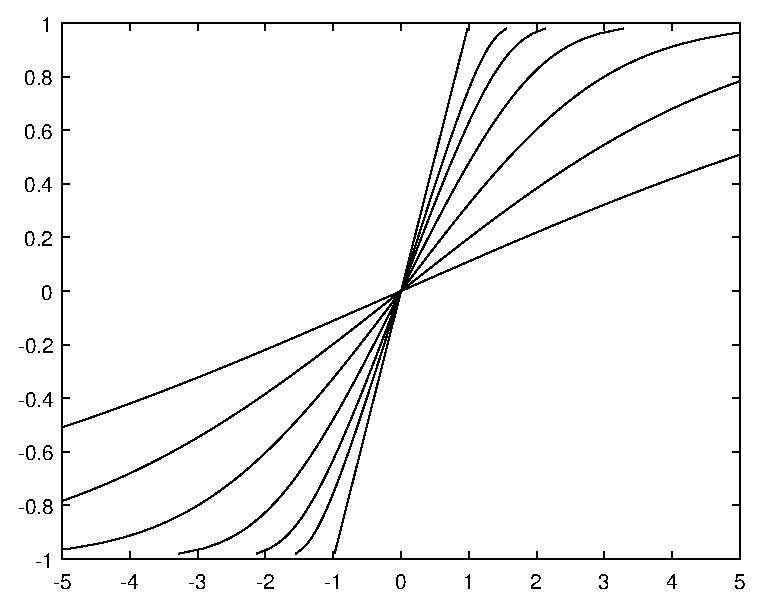
\includegraphics{projectionExample}
	\caption{Shows how the resolvent $ \res_\lambda $
		approximates the projection $ \pr_{D(A)} $ whenever
		$ \lambda\se 0 $.}
	\label{fig:example of projection}
\end{figure}

The following theorem shows that the examples generalise to all maximal monotone
operators.

\begin{theorem}\label{theorem:res is proj in limit and dom is conv}
	The set $ \overline{D(A)} $ is convex and 
	$ \res_\lambda x \ra \pr_{\overline{D(A)}} x $ 
	as $ \lambda\se 0 $ for all $ x\in\rH $.
\end{theorem}
\begin{proof}
	Define $ C:=\overline{\conv D(A)}  $ and for any $ x\in\rH $
	define $ x_\lambda:=\res_\lambda x $. First we show
	that $ x_\lambda $ is bounded as $ \lambda \se 0 $. 
	By definition of the resolvent 
	we have $ x\in x_\lambda+\lambda A x_\lambda $,
	then with the monotonicity of $ A $ we get
	for any $ (\eta,\xi)\in A $ the inequality
	\begin{align*}
		\inner{\frac{x-x_\lambda}{\lambda}-\xi}{x_\lambda-\eta}\geq 0.
	\end{align*}
	We multiply with $ \lambda $ and use the Cauchy-Schwartz inequality 
	to prove the boundedness of $ x_\lambda $ by
	\begin{align}\label{eq1:theorem:res is proj in limit and dom is conv}
		\norm{x_\lambda}^2
		\leq \inner{\lambda \xi - x}{\eta}+\inner{x_\lambda}{\eta+x-\lambda \xi}
		\leq \inner{\lambda \xi - x}{\eta}+\norm{x_\lambda}\norm{\eta+x-\lambda \xi}.
	\end{align}
	Next we show that $ x_\lambda \ra \pr_{\overline{D(A)}} x $ 
	as $ \lambda\se 0 $. 
	By lemma \ref{lemma:res is contr onto dom} we know that
	$ (x_\lambda)_{\lambda>0} $ is contained in $ D(A) $.
	As any bounded sequence in a Hilbert space has a weakly convergent
	subsequence,
	there exists a positive null-sequence $ (\lambda_n)_{n\in\NN} $ such
	that $ x_{\lambda_n} \ha x_0$ for some $ x_0 \in C $. If we apply the
	limit to \eqref{eq1:theorem:res is proj in limit and dom is conv}, 
	we get
	\begin{align}\label{eq2:theorem:res is proj in limit and dom is conv}
		\norm{x_0}^2
		\leq \limsup_{n \ra \infty}\norm{x_\lambda}^2
		=\inner{x_0}{\eta+x}-\inner{x}{\eta}
		\qimplies
		\inner{x-x_0}{\eta-x_0}
		\leq 0.
	\end{align}
	Observe the inequality on the right hand side in 
	\eqref{eq2:theorem:res is proj in limit and dom is conv}
	holds for all $ \eta \in D(A) $ and thus for all $ \eta \in C $
	(by a similar argument as in remark 
	\ref{lemma:mapped element is weak cl and conv}).
	Yet as $ C $ is closed and convex, this inequality 
	can only hold if $ x_0=\pr_{C}x $. Note that this result is independent of 
	the choice of null-sequence, which implies $ x_\lambda \ha \pr_{C}x $
	as $ \lambda \se 0 $.
	
	Lastly we must show that $ \overline{D(A)} $ is convex. 
	The same argument as above shows that the inequality on the 
	left hand side of \eqref{eq2:theorem:res is proj in limit and dom is conv}
	holds for all $ \eta\in C $. In particular if we set $ \eta=x_0 $
	in this inequality we deduce
	\begin{align}\label{eq3:theorem:res is proj in limit and dom is conv}
		\limsup_{\lambda \ra \infty}\norm{x_\lambda}^2
		= \inner{x_0}{x_0+x}-\inner{x}{x_0}
		= \norm{x_0}^2
	\end{align}
	Then \eqref{eq3:theorem:res is proj in limit and dom is conv}
	 and weak convergence is enough to imply $ x_\lambda \ra x_0 $.
	 Thus if $ x$ is in $ C $, then the sequence $ (x_\lambda)_{\lambda>0} $
	 is in $ D(A) $ and converges to $ x $. This implies $ \overline{D(A)}=C $
	 and hence $ \overline{D(A)} $ is convex.
\end{proof}

Now we introduce the Yosida approximation. A vital tool for
studying gradient flow and proper convex lower semi-continuous functions.

\begin{definition}\label{definition:Yosida Approximation}
	Let $ B $ be a maximally monotone multivalued operator in $ \rH $. 
	Define the Yosida approximation of $ B $ as the multivalued operator 
	$ B_\lambda:=\lambda^{-1}(\id-\res_\lambda) $.
\end{definition}

\begin{remark}\label{remark:triv prop yos app}
	$ \bullet $ The Yosida Approximation is a single valued operator on $ \rH $.
	\medskip
	
	$ \bullet $ The operators $ A $ and $ A_\lambda $ are 
	related for all $ x\in \rH $ by 
	$ A_\lambda x \in A \res_\lambda x $. Indeed 
	this follows from
	\begin{align*}
		A_\lambda x\in A\res_\lambda x
		\qequiv
		x\in (\id+\lambda A)\res_\lambda x 
		\qequiv
		x\in \res_\lambda^{-1}\res_\lambda x.
	\end{align*}
	
	$ \bullet $ In case $ A $ is a linear operator, then  
	$ A $ and $ A_\lambda $ are related for all 
	$ \eta\in D(A) $ by $ A_\lambda \eta=\res_\lambda A\eta $.
	The same argument as above holds, but we can replace the membership
	with an equality.
\end{remark}

\begin{definition}
	Let $ B $ be a maximally monotone multivalued operator in $ \rH $. Define the 
	minimum norm section $ B_0 $ of $ B $ to be the single valued operator with
	domain $ D(B_0)=D(B) $ and is defined by
	$ B_0 \eta := \arg\,\min_{x\in B\eta}\norm{x} $ for $ \eta\in D(B_0) $.
	This map is well-defined by lemma 
	\ref{lemma:mapped element is weak cl and conv}.
\end{definition}

We will need the following lemma a few times during this paper.

\begin{lemma}\label{lemma:weak seq cond}
	Let $ (x_n,y_n)_{n\in\NN}\subseteq A $
	be a sequence. Then we have
	$ (x,y)\in A $ if at least one of the following
	conditions is true.
	\begin{enumerate}[label=(\roman*)]
		\item We observe that $ x_n\ra x $ and $ y_n\ra y $ when $ n\ra\plus\infty $.
		\item We can verify $ x_n\ra x $ and $ y_n\ha y $ whenever $ n\ra\plus\infty $.
		\item We have that $ x_n\ha x $, $ y_n\ha y $ and 
		$ \abs{\inner{x_n}{y_n}} $ is bounded from above by 
		$ \abs{\inner{x}{y}} $ as $ n\ra\plus\infty $.
	\end{enumerate}
\end{lemma}
\begin{proof}
	We have that $ (i) $ follows from $ (ii) $, and $ (ii) $ follows from
	$ (iii) $. Indeed the first implication is clear and for the second we
	have that as $ (y_n)_{n\in\NN} $ is weakly convergent, it is 
	bounded in norm by some $ M>0 $ and thus we deduce with
	the Cauchy-Schwarz inequality
	\begin{align*}
		\abs{\inner{x_n}{y_n}-\inner{x}{y}}
		&\leq \abs{\inner{x_n-x}{y_n}}
		+\abs{\inner{x}{y_n-y}}\\
		&\leq \norm{y_n}\norm{x_n-x}
		+\abs{\inner{x}{y_n-y}}\\
		&\leq M\norm{x_n-x}
		+\abs{\inner{x}{y_n-y}}\\
		&\ra 0.
	\end{align*}
	For the property $ (iii) $, it suffices to verify the condition 
	\eqref{eq1:remark:char graph el}.
	To that end for all $ (\eta, \xi)\in A $ we compute
	\begin{align*}
		\begin{split}
			0
			\leq \limsup_{n \ra \infty}\inner{y_n-\xi}{x_n-\eta}
			&=\limsup_{n \ra \infty}\inner{y_n}{x_n}
			-\inner{\xi}{x_n}
			-\inner{y_n}{\eta}
			+\inner{\xi}{\eta}\\
			&\leq \inner{y}{x}
			-\inner{\xi}{x}
			-\inner{y}{\eta}
			+\inner{\xi}{\eta}\\
			&\leq\inner{y-\xi}{x-\eta}
		\end{split}.
	\end{align*}
\end{proof}

The Yosida Approximation has important properties, which we will use to 
construct the theory of Gradient Flows.

\begin{proposition}\label{proposition:prop of Yos app}
	Let $ A $ be a maximally monotone multivalued operator in $ \rH $. Then
	the Yosida approximation of $ A $ has the following properties
	\begin{enumerate}[label=(\roman*)]
		\item The mapping $ A_\lambda $ is $ \lambda^{-1} $-Lipschitz.
		\item The function $ A_\lambda $ is maximally monotone.
		\item We have the homomorphicity property 
		$ (A_\mu)_\lambda=A_{\mu+\lambda} $ 
		for $ \lambda,\mu >0 $.
		\item For all $ x\in D(A) $ and for any $ 0<\mu\leq \lambda $ 
		we have
		$ \norm{A_\lambda x}\leq\norm{A_\mu x}\leq \norm{A_0 x} $.
		In fact we have the estimate
		 $ \norm{ A_\lambda x- A_\mu x}^2
		\leq \norm{ A_\mu x}^2-\norm{ A_\lambda x}^2$.
		\item For all $ x\in D(A) $ we have $ A_\lambda x \ra A_0 x $ 
		when $ \lambda \se 0 $ .
		\item If $ x\notin D(A) $, then $ \norm{A_\lambda x} \ane \infty $ when 
		$ \lambda \se 0 $.
	\end{enumerate}
\end{proposition}
\begin{proof}
	"$(i)$": As $ A $ is monotone we see with the Cauchy-Schwarz inequality
	and by remark \ref{remark:triv prop yos app} for all 
	$ \eta_1,\eta_2\in\rH $ that
	\begin{align*}
		\norm{A_\lambda \eta_1-A_\lambda \eta_2}\norm{\eta_1-\eta_2}
		&\geq \inner{A_\lambda \eta_1-A_\lambda \eta_2}{\eta_1-\eta_2}\\
		&= \inner{A_\lambda \eta_1-A_\lambda \eta_2}{\lambda A_\lambda \eta_1
		-\lambda A_\lambda \eta_2+\res_\lambda \eta_1-\res_\lambda\eta_2}\\
		&= \lambda \norm{A_\lambda \eta_1-A_\lambda \eta_2}^2+
		\inner{A_\lambda \eta_1-A_\lambda \eta_2}{\res_\lambda \eta_1-\res_\lambda\eta_2}\\
		&\geq \lambda \norm{A_\lambda \eta_1-A_\lambda \eta_2}^2.
	\end{align*}
	"$ (ii) $": Suppose for some
	$ (x,y)\in\rH\times\rH $ we have
	\begin{align}\label{eq1:proposition:prop of Yos app}
		0\leq \inner{\xi-y}{\eta-x}
		\qquad \forall (\eta,\xi)\in A_\lambda.
	\end{align}
	By remark \ref{remark:triv prop yos app} we have that $ D(A_\lambda)=\rH $.
	Thus in \eqref{eq1:proposition:prop of Yos app} we get
	for all $ \eta\in\rH $ and any $ t>0 $ that
	\begin{align*}
		0
		\leq \inner{A_\lambda\big((1-t)x+t\eta\big)-y}{\big((1-t)x+t\eta\big)-x}
		= t\inner{A_\lambda((1-t)x+t\eta)-y}{\eta-x}.
	\end{align*}
	Because $ A_\lambda $ is $ \lambda^{-1} $-Lipschitz by property $ (i) $, 
	we can divide by $ t $ and take the limit $ t\se 0 $ to compute
	\begin{align*}
		0\leq \inner{A_\lambda x-y}{\eta-x}.
	\end{align*}
	As this inequality must hold for all $ \eta\in\rH $, we deduce that 
	$ A_\lambda x=y $. 
	This proves that $ A_\lambda  $
	is maximally monotone.\smallskip
	
	"$ (iii) $": The claim is an immediate consequence of the following equivalence chain
	\begin{align*}
		(\eta,\xi)\in A_\lambda
		\sequiv
		\res_\lambda \eta=\eta-\lambda \xi 
		\sequiv
		\eta\in (\eta-\lambda \xi)+\lambda A(\eta-\lambda \xi)
		\sequiv
		(\eta-\lambda \xi, \xi)\in A.
	\end{align*}
	"$ (iv) $":  
	For $ 0<\mu<\lambda $ and by remark \ref{remark:triv prop yos app} 
	we compute using the monotonicity of $ A $ and the Cauchy-Schwarz inequality
	\begin{align*}
		\begin{split}
			\inner{A_0 x - A_{\lambda-\mu} x}{x-\res_{\lambda-\mu} x}\geq 0
			&\simplies
			\inner{A_0 x - A_{\lambda-\mu} x}{A_{\lambda-\mu} x}\geq 0\\
			&\simplies
			\norm{A_0 x}\norm{A_{\lambda-\mu} x}
			\geq \inner{A_0 x}{A_{\lambda-\mu} x}
			\geq \norm{A_{\lambda-\mu} x}^2.
		\end{split}
	\end{align*}
	We extract the following inequalities which are of interest to us
	\begin{align}
		\norm{A_{\lambda-\mu} x} 
		&\leq \norm{A_0 x},
		\label{eq2:proposition:prop of Yos app}\\
		\norm{A_{\lambda-\mu} x}^2
		&\leq \inner{A_0 x}{A_{\lambda-\mu} x}.
		\label{eq3:proposition:prop of Yos app}
	\end{align}
	Now we show the first bound of $ (iv) $.
	From \eqref{eq2:proposition:prop of Yos app}
	we can easily see that $ \norm{A_\mu x}\leq\norm{A_0 x} $.
	Note that $ (A_\mu)_0=A_{\mu} $ as $ A_\mu $ is single valued from 
	remark \ref{remark:triv prop yos app}. So we may replace $ A $ with $ A_\mu $ 
	in \eqref{eq2:proposition:prop of Yos app}
	and use property $ (iii) $ to get $ \norm{A_\lambda x}\leq \norm{A_\mu x} $. 
	\smallskip
	
	For the second bound in $ (iv) $, we argue analogue
	as before and transform
	\eqref{eq2:proposition:prop of Yos app}
	into the inequality $ \inner{A_\lambda x}{A_\mu x}\leq \norm{A_\lambda x}^2 $.
	Then we get the desired inequality
	\begin{align*}
		\norm{ A_\lambda x- A_\mu x}^2
		&=\norm{ A_\lambda x}^2+\norm{A_\mu x}^2-2\inner{A_\lambda x}{A_\mu x}
		\leq \norm{A_\mu x}^2+\norm{ A_\lambda x}^2-2\norm{A_\lambda x}^2.
	\end{align*}
	
	"$(v)$": Property $ (iv) $ tells us that $ \norm{A_\lambda x} $
	is monotonically increasing as $ \lambda\se 0 $ with upper
	bound $ \norm{A_0 x} $. This fact coupled with the second
	property $ (iv) $ shows that the sequence $ (A_\lambda x)_{\lambda>0} $ is
	Cauchy and hence strongly converges to some $ y\in\rH $
	with $ \norm{y}\leq \norm{A_0 x} $.
	Moreover by theorem
	\ref{theorem:res is proj in limit and dom is conv}
	as $ x\in D(A) $ we have that $ \res_\lambda x\ra \pr_{\overline{D(A)}} x =x$,
	and by remark \ref{remark:triv prop yos app} we have a sequence 
	$ (\res_\lambda x,A_\lambda x)_{\lambda >0}\subseteq A $.
	Thus by lemma \ref{lemma:weak seq cond} we see that $ (x,y)\in A $.
	By definition of the minimum norm section and as $ \norm{y}\leq \norm{A_0 x} $
	we must have $ y=A_0 x $.\medskip
	
	"$ (vi) $": We show the contra-positive. So suppose that the
	sequence $ \norm{A_\lambda x} $ is bounded as $ \lambda \se 0 $.
	As an immediate consequence we get
	 $ x-\res_\lambda x=\lambda A_\lambda x\ra 0 $.
	 Then by theorem \ref{theorem:res is proj in limit and dom is conv} 
	 we have that $ \res_{\lambda_n} x \ra \pr_{\overline{D(A)}} x=x$.
	There must exist some positive null-sequence $ \lambda_n\ra 0 $
	and $ y\in\rH $ such that $ A_{\lambda_n} x\ha y $. 
	Then by lemma \ref{lemma:weak seq cond}
	we have $ (x,y)\in A $.
	In particular we derive that $ x\in D(A) $ thus proving the property $ (vi) $.
\end{proof}

\subsection{Proper Convex Lower Semicontinous Potentials in Hilbert Spaces}

In this section we analyse an important class of maximal monotone operators,
namely the sub differentials of proper convex lower semicontinous
functions in a Hilbert Space.\medskip

For any mapping $ \varphi:\rH \ra \eRR $ we define its domain $ D(\vp) $
by the set $ \{x\in\rH\sep\vp(x)\neq\plus\infty \} $.

\begin{definition}
	A mapping $ \varphi:\rH \ra \eRR $ is called a proper convex function 
	if it satisfies
	\begin{enumerate}[label=(\roman*)]
		\item The domain of $ \vp $ is non-empty, i.e. $ D(\vp)\neq\emptyset $.
		\item For all $ x,y\in D(\vp) $ 
		and all $ 0<\lambda<1 $ we have 
		$ \vp(\lambda x+(1-\lambda)y)\leq \lambda\vp(x)+(1-\lambda)\vp(y) $.
	\end{enumerate}
\end{definition}

\begin{remark}\label{remark:dom of prop conv fun is conv}
	Any proper convex function $ \varphi:\rH \ra \eRR $
	is complemented with a convex domain. Indeed this is an immediate
	consequence of the definition.
\end{remark}

\begin{definition}
	A function $ \varphi:\rH \ra \eRR $ is lower semi-continuous (l.s.c) if 
	it satisfies the lower continuity condition, i.e. if it satisfies
	\begin{align*}
		\forall x\in D(\vp)\,
		\forall \eta>0\,
		\exists\delta>0\,
		\forall y\in D(\vp)
		\quad :\;
		\norm{x-y}<\delta
		\implies 
		f(x)-\varepsilon<f(y).
	\end{align*}
\end{definition}

\begin{remark}\label{remark:lim inf prop lsc}
	Let $ \varphi:\rH \ra \eRR $ be a l.s.c. function, 
	$ (x_n)_{n\in\NN}\in D(\vp) $ a sequence with limit $ x\in D(\vp) $.
	As an immediate consequence of the definition 
	we have the following limit behaviour 
	\begin{align*}
		\vp(x)\leq \liminf_{n\ra \infty}\vp(x_n).
	\end{align*} 
\end{remark}

\begin{remark}\label{remark:prop lsc func is sup of aff}
	%TODO find source
	From \cite{rockafellar2015convex}
	we know that for every proper lower semi-continuous function 
	$ \vp:\rH\ra(\minus\infty,\plus\infty] $ 
	there exists a family of affine functions
	$ \ell_i(x):=\inner{v_i}{x}+b_i $ for
	$ i\in I $, $ v_i\in\rH $, $ b_i\in\RR $ and every 
	$ x\in\rH $, such that 
	\begin{align*}
		\vp(x)=\sup_{i\in I}\ell_i(x)
		\qquad\forall x\in\rH.
	\end{align*}
\end{remark}

\begin{definition}
	For any proper convex l.s.c function $ \varphi:\rH \ra \eRR $ we
	define the sub differential mapping $ \prt\vp $ of $ \vp $
	as the multivalued operator in $ \rH $ with the graph defined by
	\begin{align*}
		\prt\vp:=\{(\eta,\xi)\in D(\vp)\times\rH
		\sep \forall x\in D(\vp)\;:\;\vp(x)\geq \vp(\eta)+\inner{\xi}{x-\eta}\,\}.
	\end{align*}
\end{definition}

\begin{remark}
	From the definition we have that $ D(\prt\vp)\subseteq D(\vp) $.
\end{remark}

In other literature a proper convex l.s.c mapping
$ \vp:\rH\ra(\minus\infty,\plus\infty] $ is also
called a potential on $ \rH $. We can show that the sub 
differential mapping is a multivalued 
maximal monotone operator in $ \rH $. This follows from the next two lemmas.

\begin{lemma}\label{lemma:sub diff is mon}
	The sub differential $ \prt \vp $ of a proper convex l.s.c.
	function $ \varphi:\rH \ra \eRR $ is monotone.
\end{lemma}
\begin{proof}
	We have for all $ (\eta_1,\xi_1), (\eta_2, \xi_2)\in \prt \vp $
	by definition of the sub differential
	\begin{align*}
		\vp(\eta_2)&\geq \vp(\eta_1)+\inner{\xi_1}{\eta_2-\eta_1},\\
		\vp(\eta_1)&\geq \vp(\eta_2)+\inner{\xi_2}{\eta_1-\eta_2}.
	\end{align*}
	We can reformulate these inequalities as
	\begin{align*}
		\inner{\xi_1}{\eta_1-\eta_2}&\geq \phantom{-(}\vp(\eta_1)-\vp(\eta_2),\\
		\inner{-\xi_2}{\eta_1-\eta_2}&\geq -(\vp(\eta_1)-\vp(\eta_2)).
	\end{align*}
	We prove the claim by taking the sum of these inequalities since
	\begin{align*}
		\inner{\xi_1-\xi_2}{\eta_1-\eta_2}\geq 0.
	\end{align*}
\end{proof}

\begin{lemma}\label{lemma:cond prop conv. l.s.c. sub diff}
	Let $ \vp:\rH \ra \eRR $ be a proper convex l.s.c.
	function, pick any $ \alpha > 0 $ and let
	$ \eta,\xi\in\rH $. Then the mapping $ \psi:\rH \ra \eRR;\, 
	x\mapsto \vp(x)+\frac{\alpha}{2}\norm{x-\xi}^2$
	attains its minimal value at $ \eta $ if and only if
	$ \alpha(\xi-\eta) \in \prt \vp(\eta) $.
\end{lemma}
\begin{proof}
	Suppose first that the mapping $ \psi $ attains its minimal value at
	$ \eta $. Then for all $ x\in\rH $ and all $ 0<t<1 $ we have
	by the monotonicity of $ \vp $ that
	\begin{align*}
		t(\vp(x)-\vp(\eta))
		&\geq \vp\big((1-t)\eta+tx\big)-\vp(\eta)\\
		&\geq \frac{\alpha}{2}\norm{\eta-\xi}^2
		-\frac{\alpha}{2}\norm{(1-t)\eta+tx-\xi}^2\\
		&= \frac{\alpha}{2}\norm{\eta-\xi}^2
		-\frac{\alpha}{2}\norm{t(x-\eta)+\eta-\xi}^2\\
		&\geq -t^2\frac{\alpha}{2}\norm{x-\eta}^2
		-t\alpha\inner{x-\eta}{\eta-\xi}.
	\end{align*}
	If we divide by $ t $ and take the limit $ t\se 0 $, 
	we prove $ \alpha(\xi-\eta)\in\prt\vp(\eta) $ by
	\begin{align*}
		\vp(x)-\vp(\eta)
		\geq -\alpha\inner{x-\eta}{\eta-\xi}
		\qimplies
		\vp(x)
		\geq \vp(\eta)+\inner{\alpha(\xi-\eta)}{x-\eta}.
	\end{align*}

	Now assume that the converse holds true, i.e.
	$ \alpha(\xi-\eta)\in\prt\vp(\eta) $. Then $ \psi $ is has
	a minimum at $ \eta $ by the following computation
	\begin{align*}
		\begin{split}
			\vp(x)-\vp(\eta)
			&\geq \alpha\inner{\xi-\eta}{x-\eta}\\
			&\geq \alpha\inner{\xi-\eta}{x-\eta}-\frac{\alpha}{2}\norm{x-\eta}^2\\
			&=\frac{\alpha}{2}\norm{\eta-\xi}^2-\frac{\alpha}{2}\norm{x-\xi}^2.
		\end{split}
		\qquad
		\forall x\in \rH.
	\end{align*}
\end{proof}

\begin{corollary}\label{corollary:sub diff of pr lsc func is max mon op}
	The sub differential $ \prt \vp $ of a proper convex l.s.c.
	function $ \varphi:\rH \ra \eRR $ is maximally monotone.
\end{corollary}
\begin{proof}
	From lemma \ref{lemma:sub diff is mon} 
	we know that $ \prt\vp $ is monotone.
	So by proposition \ref{proposition:criteria for max mon}
	it suffices to prove that $ R(\id+\prt \vp)=\rH $.
	Note that the function $\psi: \rH \ra \eRR;\, 
	x\mapsto \vp(x)+\frac{1}{2}\norm{x-\xi}^2$ diverges towards
	$ \plus\infty $ as $ \norm{x}\ra\plus\infty $
	for all $ \xi\in\rH $. Indeed 
	this is clear if $ \vp $ is an affine function. Then by 
	remark \ref{remark:prop lsc func is sup of aff}
	the claim holds for any l.s.c. proper convex function.
	Therefore $ \psi $ has some minimal value $ \eta\in D(\vp) $.\smallskip
	
	But by lemma \ref{lemma:cond prop conv. l.s.c. sub diff}
	we know that $ \eta $ is a minimal value of $ \psi $
	if and only if $ \xi-\eta \in \prt \vp(\eta) $. This means
	that $ \xi \in \eta + \prt \vp(\eta) $ from which follows the claim.
\end{proof}

We will need an elementary lemma for the next proposition,
characterizing the convexity of a differentiable
function on $ \RR $ by its first derivative.
We will only state the lemma and not the proof,
as it is only tangentially related to the subject.

\begin{lemma}\label{lemma:der of conv fun is mon inc}
	Let $ \vp:\RR\ra\RR $ be a differentiable function, then we have that
	$ \prt_t f $ is monotonically increasing if and only if 
	$ f $ is convex.
\end{lemma}

The upcoming proposition shows that the Yosida approximation
of the sub differential operator of a proper convex l.s.c
function, is the sub differential of 
a Fréchet differentiable convex function on $ \rH $. 

\begin{proposition}\label{proposition:yosida approx of prop lsc conv}
	Let $\vp$ be proper convex l.s.c. mapping on $ \rH $ and
	define $ A:=\prt \vp $. Then for all $ \lambda>0 $ define
	the function
	\begin{align}\label{equation:yosida potential formal def}
		\vp_\lambda(x)
		=\min_{y\in \rH}\,\frac{1}{2\lambda}\norm{x-y}^2+\vp(y).
	\end{align}
	This function has the following properties
	\begin{enumerate}[label=(\roman*)]
		\item The function $ \vp_\lambda $ has an equivalent formulation
		\begin{align}\label{equation:yosida potential res def}
			\vp_\lambda(x)=\frac{\lambda}{2}\norm{A_\lambda x}^2
			+\vp(\res_\lambda x),
		\end{align}
		\item The map $ \vp_\lambda $ is Fréchet-differentiable
		with derivative $ \prt_x\vp_\lambda(x)y=\inner{A_\lambda x}{y} $.
		Moreover the sub differential of $ \vp_\lambda $ coincides with
		the Yosida approximation $ A_\lambda $, i.e 
		$ (\prt\vp_\lambda)_\lambda=A_\lambda $.
		\item  The function $ \vp_\lambda $ is convex function with domain $ \rH $. 
		\item We have that $ \vp_\lambda(x)\ane \vp(x) $ whenever 
		$ \lambda\se 0 $ for all $ x\in \rH $.  
		\item The domain of $ \vp $ and $ A $ are related by 
		$ \overline{D(\vp)}=\overline{D(A)} $.
	\end{enumerate}
\end{proposition}
\begin{proof}
	First we tackle the property $ (i) $.
	By remark \ref{remark:triv prop yos app} we have 
	$ \frac{1}{\lambda}(x-\res_\lambda x)=A_\lambda x\in A\res_\lambda x$.
	Then if in lemma \ref{lemma:cond prop conv. l.s.c. sub diff}
	we set $ \alpha=\lambda^{-1} $, $ \xi=x$ and $\eta=\res_\lambda x $, 
	we have that 
	the map $ \rH\ra\eRR;\,y \mapsto  \frac{1}{2\lambda}\norm{x-y}^2+\vp(y)$
	attains its minimal value at $\res_\lambda x$, 
	thus proving the alternate definition of $ \vp_\lambda $
	in \eqref{equation:yosida potential res def}.\smallskip
	
	Next we verify that $ \vp_\lambda $ is Fréchet differentiable. For all
	$ x,y\in D(\vp) $ note by \eqref{equation:yosida potential res def} that
	\begin{align*}
		\vp_\lambda(x)-&\vp_\lambda(y)\\
		&=\frac{\lambda}{2}(\norm{A_\lambda x}^2-\norm{A_\lambda y}^2)+\vp(\res_\lambda x)-\vp(\res_\lambda y)\\
		&\geq \frac{\lambda}{2}(\norm{A_\lambda x}^2-\norm{A_\lambda y}^2)+\inner{A_\lambda y}{\res_\lambda x-\res_\lambda y}\\
		&=\frac{\lambda}{2}(\norm{A_\lambda x}^2-\norm{A_\lambda 
		y}^2)
		+\inner{A_\lambda y}{y-\res_\lambda y}
		-\inner{A_\lambda y}{x-\res_\lambda x}
		+\inner{A_\lambda y}{x-y}\\
		&=\frac{\lambda}{2}\Big(\norm{A_\lambda x}^2-\norm{A_\lambda 
			y}^2+2\inner{A_\lambda y}{A_\lambda y-A_\lambda x}\Big)
		+\inner{A_\lambda y}{x-y}.
	\end{align*}
	We reorder the inequality and continue
	\begin{align}\label{eq1:proposition:yosida approx of prop lsc conv}
		\begin{split}
			\vp_\lambda(x)-\vp_\lambda(y)-&\inner{A_\lambda y}{x-y}\\
			&\geq \frac{\lambda}{2}\big(\norm{A_\lambda x}^2-\norm{A_\lambda 
				y}^2+2\inner{A_\lambda y}{A_\lambda y-A_\lambda x}\big)\\
			&=\frac{\lambda}{2}\big(\norm{A_\lambda x-A_\lambda y}^2
			+2\inner{A_\lambda x-A_\lambda y}{A_\lambda y}
			+2\inner{A_\lambda y}{A_\lambda y-A_\lambda x}\big)\\
			&=\frac{\lambda}{2}\norm{A_\lambda x-A_\lambda y}^2\\
			&\geq 0.
		\end{split}
	\end{align} 
	We may swap $x$ and $y$ and negate to get 
	$\vp_\lambda(x)-\vp_\lambda(y)-\inner{A_\lambda x}{x-y}\leq 0 $.
	By restructuring this inequality we see
	\begin{align}\label{eq2:proposition:yosida approx of prop lsc conv}
		\vp_\lambda(x)-\vp_\lambda(y)-\inner{A_\lambda y}{x-y}
		\leq \inner{A_\lambda x-A_\lambda y}{x-y}.
	\end{align}
	From preposition \ref{proposition:prop of Yos app} we know that
	$ A_\lambda $ is $ \lambda^{-1} $-Lipshitz. Thus
	by using both \eqref{eq1:proposition:yosida approx of prop lsc conv}
	and \eqref{eq2:proposition:yosida approx of prop lsc conv}
	and  the Cauchy-Schwarz inequality wee see that
	\begin{align*}
		\abs{\vp_\lambda(x)-\vp_\lambda(y)-\inner{A_\lambda y}{x-y}}
		\leq \inner{A_\lambda x-A_\lambda y}{x-y}
		\leq \frac{1}{\lambda}\norm{x-y}^2.
	\end{align*}
	This shows that $ \vp_\lambda $ is Fréchet differentiable in $ D(\vp) $ with
	derivative $ \partial_x\vp_\lambda(x)y= \inner{A_\lambda x}{y} $
	for all $ x\in D(\vp) $ and $ y\in\rH $.\smallskip
	
	Now we show property $ (iv) $. By lemma \ref{lemma:der of conv fun is mon inc}
	it suffices
	to show for all $\eta_1,\eta_2\in D(\vp)$ that the mapping
	$ (0,1)\ra\RR;\,t\mapsto \prt_t\vp_\lambda(t \eta_1+(1-t)\eta_2) $
	is monotonically increasing. By proposition \ref{proposition:prop of Yos app}
	we know that $ A_\lambda $ is monotone. Thus for all $ 0<s\leq t<1 $ we have
	\begin{align*}
		\big(\prt_t \vp_\lambda(t \eta_1+&(1-t)\eta_2)
		-\prt_t \vp_\lambda(s \eta_1+(1-s)\eta_2)\big)\cdot(t-s)\\
		&=\inner{A_\lambda(t \eta_1+(1-t)\eta_2)
			-A_\lambda(s \eta_1+(1-s)\eta_2)}{\eta_1-\eta_2}\cdot(t-s)\\
		&=\inner{A_\lambda(\eta_2+t(\eta_1-\eta_2))
			-A_\lambda(\eta_2+s(\eta_1-\eta_2))}{
			\eta_2+t(\eta_1-\eta_2)-(\eta_2+s(\eta_1-\eta_2))}\\
		&\geq 0.
	\end{align*}
	Next we show statement $ (v) $. 
	From the two function definitions \eqref{equation:yosida potential formal def} 
	and \eqref{equation:yosida potential res def}
	we see that $ \vp_\lambda(x) $ monotonically
	increases as $ \lambda $ decreases and that 
	$ \vp(\res_\lambda x)\leq \vp_\lambda(x)\leq \vp(x) $. 
	For any $ \eta\in\overline{D(A)} $ we have by 
	theorem \ref{theorem:res is proj in limit and dom is conv}
	that $ \res_\lambda\eta\ra\eta $ as $ \lambda\se 0 $. 
	Then by remark \ref{remark:lim inf prop lsc}
	we have
	\begin{align*}
		\vp(x)
		\leq\liminf_{\lambda\se 0} \vp(\res_\lambda x)
		\leq\liminf_{\lambda\se 0} \vp_\lambda(x)
		\leq\limsup_{\lambda\se 0} \vp_\lambda(x)
		\leq \vp(x).
	\end{align*}
	This shows that $ \vp_\lambda(\eta)\ane\vp(\eta) $
	when $ \lambda\se 0 $. If $ x\notin \overline{D(A)} $,
	then $ x-\res_\lambda x\ra x-\pr_{D(A)} x\neq 0 $. As $ \vp $
	is lower semi continuous, there exists a neighborhood
	of $ 0 $ and some constant $ C\in\RR $
	such that for all $ \lambda >0 $ sufficiently small
	we have $ \vp(\res_\lambda x)\geq C $. In conjunction
	we observe a divergence
	\begin{align*}
		\liminf_{\lambda\ra 0}\vp_\lambda(x)
		=\liminf_{\lambda\ra 0}\frac{\lambda}{2}\norm{A_\lambda x}^2
		+\vp(\res_\lambda x)
		\geq \liminf_{\lambda\ra 0}\
		\frac{1}{2}\norm{A_\lambda x}\norm{x-\res_\lambda x}+C
		=\plus\infty.
	\end{align*}
	The last property $ (v) $ is an immediate 
	consequence, since we have just
	deduced that $ D(\vp)\subseteq\overline{D(A)} $,
	and thus $ \overline{D(\vp)}=\overline{D(A)} $.
\end{proof}